\documentclass[a4paper,11pt]{article}
\usepackage[spanish]{babel}
\usepackage[utf8]{inputenc}

% Configuración páginas
\usepackage{vmargin}							% Márgenes

\usepackage{sectsty}							% Fuente de los títulos
\allsectionsfont{\normalfont \Large \scshape}

\usepackage{graphicx}							% Imágenes
\graphicspath{{images/}}

\usepackage{tabularx}							% Otras
\usepackage{multirow}							% Celdas ocupando varias filas

\usepackage{mathtools}							% Matematicas
\newcommand\numberthis{							% numeración en align*
	\addtocounter{equation}{1}\tag{\theequation}
}

\usepackage{algorithm,algpseudocode}			% Algoritmos en latex
\makeatletter
\renewcommand{\ALG@name}{Algoritmo}				% Cambiamos la palabra "Algorithm"
\makeatother
\algnewcommand\Input{\item[\textbf{Entrada:}]}
\let\oldReturn\Return
\renewcommand{\Return}{\State\oldReturn}

% Configuración del título
\newcommand{\horrule}[1]{\rule{\linewidth}{#1}} 	% Horizontal rule

\title{
	\vspace{-25pt}
	\normalfont \Large \textsc{
		Modelos de Investigación Operativa,
        Ingeniería Informática\\
        Universidad de Valladolid
	}\\[10pt]
	\horrule{1pt}\\[10pt]
	\huge \textbf{
		Práctica 13
	}\\
	\horrule{1pt}
}
\author{
	\normalfont \Large Daniel González Alonso
}
\date{
	\normalfont \large \today
}

%%%%%%%%%%%%%%%%%%%%%%%%%%%%%%%%%%%%%%%%%%%%%%%%%%
\begin{document}
\maketitle

%%%% RESUMEN %%%%
\begin{abstract}
	En este documento se describen los problemas y los resultados obtenidos de la práctica 13 del tema 5 de la asignatura Modelos de Investigación Operativa de Ingeniería Informática, Universidad de Valladolid.
\end{abstract}

%%%% DESARROLLO %%%%
\section{Introducción}
Esta práctica trata de problemas TSP (\textit{Travelling Salesman Problem}). Los problemas TSP constan de un grafo ${G=(N,A)}$, donde ${N}$ son los nodos del grafo y ${A}$ los arcos entre éstos, con un coste asociado por cada arco, y el objetivo consiste en encontrar el camino Hamiltoniano (un camino que pase por todos los nodos) de coste mínimo.\\

En esta práctica se nos pide implementar la solución al problema TSP mediante la metaheurística \textit{Simulated Annealing} para TSP. El pseudocódigo de la esta metaheurística se muestra a continuación:

\begin{algorithm}[!htbp]
\caption{Metaheurística \textit{Simulated Annealing}}
\label{alg_sim_annealing}
\begin{algorithmic}[1]
\Function{SimulatedAnnealing}{${T_{0}, X}$}
	\State ${T \gets T_{0}}$
    \State ${x_{1} \gets \Call{GenerarSolucionInicial}{X}}$
    \State ${x^{\ast} \gets x_{1}}$, ${F^{\ast} \gets F(x_{1})}$
    \State ${flag = 0}$
    \While{Condición de parada no se satisfaga}
		\State ${x \gets \Call{GenerarSolucionEnEntorno}{x_{n}}}$
        \If{${F(x) \leq F(x_{n})}$}
        	\State ${x_{n} \gets x}$
        \EndIf
        \algstore{alg_sim_annealing}
\end{algorithmic}
\end{algorithm}

\newpage
\begin{algorithm}[!htbp]
\begin{algorithmic}[1]
		\algrestore{alg_sim_annealing}
        \If{${F^{\ast} < F(x_{n})}$}
        	\State ${x^{\ast} \gets x}$, ${F^{\ast} \gets F(x)}$
        \Else
        	\State ${p \gets \Call{random}{}}$	\Comment{Generar número aleatorio en [0,1]}
            \If{${p \leq p(n)}$}
            	\State ${x_{n} \gets x}$
            \EndIf
        \EndIf
        \State ${\Call{Disminuir}{T}}$
    \EndWhile
	\Return{${x^{\ast}}$}
\EndFunction
\end{algorithmic}
\end{algorithm}

En nuestro caso, para la función ${\Call{GenerarSolucionInicial}{X}}$ se ha empleado la heurística del entorno más cercano. Para la función ${\Call{GenerarSolucionEnEntorno}{x_{n}}}$ se elegían aleatoriamente dos nodos ${i}$ y ${j}$ no contiguos, y se hacía el intercambio explicado en la práctica 11. Para calcular el valor de ${p_{n}}$ se empleaba la siguiente fórmula:

\begin{equation}
\label{formula_p_n}
p_{n} = \exp{\left( -\frac{\Delta_{i,j}}{T_{n}} \right)}
\end{equation}

Donde ${\Delta_{i,j}}$ es la mejora del intercambio de la solución ${x}$ respecto a ${x_{n}}$. Por otro lado para la función ${\Call{Disminuir}{T}}$, es decir la disminución de la temperatura, se escogió la disminución lineal, la cual sigue la función 

\begin{equation}
\label{formula_t_n}
T_{n+1} = \alpha \cdot T_{n}
\end{equation}

Siendo el valor ${\alpha}$ una constante a definir. Por último como condición de parada se eligió tanto limitar el número máximo de iteraciones, como limitar el número máximo de iteraciones sin mejora ${K}$.


%%%%%%%%%%%%%%%%%%%%%%%%%%%%%%%%%%%%%%%%%%%%%%%%%%%%%%
\newpage
\section{Desarrollo}
En esta práctica hay que programar la heurística \textit{Simulated Annealing} y aplicarla a los 5 ejemplos de ${n=21}$ nodos y los 6 problemas Euclídeos de las prácticas anteriores.\\

Estos problemas se encuentran resueltos mediante \textit{Xpress Mosel} en los ficheros \texttt{tsp\_sa\_ \ n21\_1.mos}, \texttt{tsp\_sa\_n21\_2.mos}, \texttt{tsp\_sa\_n21\_3.mos}, \texttt{tsp\_sa\_n21\_4.mos}, \texttt{tsp\_sa\_n21\_5.mos} en el caso de los ficheros \texttt{n21} y por otro lado para los ficheros \texttt{tsp} Euclídeos en los ficheros \texttt{tsp\_sa\_tsp\_60\_1.mos}, \texttt{tsp\_sa\_tsp\_60\_2.mos}, \texttt{tsp\_sa\_tsp\_60\_3.mos}, \texttt{tsp\_sa\_tsp\_100\_1.mos}, \texttt{tsp\_sa\_tsp\_100\_2.mos} y \texttt{tsp\_sa\_tsp\_100\_3.mos} (el nombre indica el fichero de datos empleado).\\

Antes de explicar la implementación del algoritmo cabe destacar que los costes ${c_{i,j}}$ en nuestro caso son distancias. Para los ficheros \texttt{n21} la matriz de distancias nos viene dada en el mismo fichero. En el caso de los ficheros \texttt{tsp} solo nos vienen las coordenadas de cada nodo, por ello antes de empezar con estos últimos ficheros hay que calcular la matriz de distancias. Para estos fichero la matriz se calculo mediante la distancia Euclídea redondeada al entero más cercano. En caso de la distancia de un nodo a si mismo, se introducía en esta matriz en vez de 0 un valor ``infinito'' (\texttt{MAX\_INT}).\\

Para el algoritmo \textit{Simulated Annealing} como se ha explicado en el esquema anterior lo primero que hay que obtener es una solución inicial, y como se hay dicho se empleó la heurística del entorno más cercano, ya implementado en la práctica 10.\\

Posteriormente, ya dentro del bucle principal, los pasos que se hicieron siguiendo el esquema \ref{alg_sim_annealing} fueron los siguientes:

\begin{enumerate}
\item Generar solución en el entorno de la solución actual: Para esta parte, simplemente elegía dos nodos aleatoriamente, y después al igual que se hizo en la práctica 11 con el algoritmo \textit{2-opt}, se intercambia los arcos ${(i,s(i))}$ y ${(j,s(j))}$ por ${(i,j}$ y ${(s(i),s(j))}$, y se invertía de dirección el camino entre ellos. Además también se calculaba el valor ${\Delta_{i,j}}$ para obtener la distancia total de la solución actual.
\item Actualizar la solución óptima: en este caso simplemente reemplazaríamos el vector \texttt{siguientes} y la \texttt{distancia\_minima} por la de la solución actual en caso de que su distancia fuese inferior.
\item Actualizar la solución ${x_{n}}$: en este caso, al igual que en el paso anterior si la solución actual fuese mejor o igual reemplazaríamos su vector de siguientes y la distancia. Si no fuese menor o igual, lo reemplazaríamos con probabilidad ${p}$ basándonos en la fórmula \ref{formula_p_n}.
\item Actualizar ${T\_{n}}$: Para esta parte simplemente aplicamos la fórmula \ref{formula_t_n}. En el caso de los ficheros \texttt{n21} empleó un valor de ${\alpha = 0.961}$, ${\alpha = 0.931}$ para los ficheros \texttt{tsp\_60} y ${\alpha = 0.91}$ para los fichero \texttt{tsp\_100}.
\item Actualizar la condición de parada: para la condición de parada utilizamos una bandera, la cual pararía el bucle en caso de que se alcanzase un máximo número de iteraciones sin mejorar (${K=58000}$ en el caso de los ficheros \texttt{n21}, ${K=65000}$ para \texttt{tsp\_60} y ${K=2000000}$ para \texttt{tsp\_100}) la solución o un máximo número de iteraciones.
\end{enumerate}

%%%%%%%%%%%%%%%%%%%%%%%%%%%%%%%%%%%%%%%%%%%%%%%%%%%%%%
\newpage
\section{Resultados}
Los resultados obtenidos para los ficheros de datos de esta práctica fueron los siguientes:

\begin{table}[!htbp]
\label{results_n21}
\centering
\begin{tabularx}{\textwidth}{|p{2cm}|X|X|X|X|X|}
\hline
Problema TSP  & \texttt{n21\_1}	& \texttt{n21\_2}	& \texttt{n21\_3}	& \texttt{n21\_4}	& \texttt{n21\_5}	\\ \hline
Distancia Total & 243	& 234	& 227	& 231	& 253	\\ \hline
Conexiones & 1 $\to$ 8 $\to$ 14 $\to$ 4 $\to$ 15 $\to$ 3 $\to$ 16 $\to$ 2 $\to$ 6 $\to$ 12 $\to$ 9 $\to$ 11 $\to$ 13 $\to$ 19 $\to$ 18 $\to$ 20 $\to$ 10 $\to$ 17 $\to$ 7 $\to$ 21 $\to$ 5	& 1 $\to$ 2 $\to$ 11 $\to$ 10 $\to$ 20 $\to$ 8 $\to$ 4 $\to$ 21 $\to$ 13 $\to$ 18 $\to$ 16 $\to$ 12 $\to$ 17 $\to$ 7 $\to$ 6 $\to$ 5 $\to$ 9 $\to$ 19 $\to$ 3 $\to$ 15 $\to$ 14	& 1 $\to$ 7 $\to$ 6 $\to$ 20 $\to$ 19 $\to$ 13 $\to$ 12 $\to$ 18 $\to$ 15 $\to$ 16 $\to$ 8 $\to$ 3 $\to$ 5 $\to$ 17 $\to$ 10 $\to$ 9 $\to$ 11 $\to$ 2 $\to$ 21 $\to$ 4 $\to$ 14	& 1 $\to$ 4 $\to$ 13 $\to$ 21 $\to$ 12 $\to$ 5 $\to$ 17 $\to$ 18 $\to$ 19 $\to$ 16 $\to$ 10 $\to$ 8 $\to$ 3 $\to$ 20 $\to$ 11 $\to$ 15 $\to$ 14 $\to$ 7 $\to$ 6 $\to$ 2 $\to$ 9	& 1 $\to$ 7 $\to$ 10 $\to$ 16 $\to$ 15 $\to$ 5 $\to$ 11 $\to$ 6 $\to$ 3 $\to$ 18 $\to$ 13 $\to$ 19 $\to$ 21 $\to$ 4 $\to$ 2 $\to$ 9 $\to$ 17 $\to$ 8 $\to$ 20 $\to$ 14 $\to$ 12	\\ \hline
\end{tabularx}
\caption{Resultados obtenidos para los ficheros \texttt{n21}}
\end{table}

\begin{table}[!htbp]
\label{results_tsp_60}
\centering
\begin{tabularx}{\textwidth}{|p{2cm}|X|X|X|}
\hline
Problema TSP    & \texttt{tsp\_60\_1}   & \texttt{tsp\_60\_2}   & \texttt{tsp\_60\_3}	\\ \hline
Distancia Total & 837	& 709	& 732	\\ \hline
Conexiones    & 1 $\to$ 35 $\to$ 53 $\to$ 27 $\to$ 23 $\to$ 32 $\to$ 8 $\to$ 12 $\to$ 20 $\to$ 51 $\to$ 54 $\to$ 39 $\to$ 31 $\to$ 50 $\to$ 58 $\to$ 49 $\to$ 40 $\to$ 60 $\to$ 14 $\to$ 37 $\to$ 18 $\to$ 29 $\to$ 4 $\to$ 34 $\to$ 16 $\to$ 25 $\to$ 19 $\to$ 9 $\to$ 43 $\to$ 47 $\to$ 55 $\to$ 28 $\to$ 56 $\to$ 5 $\to$ 42 $\to$ 48 $\to$ 36 $\to$ 11 $\to$ 44 $\to$ 59 $\to$ 3 $\to$ 33 $\to$ 45 $\to$ 52 $\to$ 24 $\to$ 41 $\to$ 38 $\to$ 17 $\to$ 2 $\to$ 7 $\to$ 21 $\to$ 15 $\to$ 26 $\to$ 6 $\to$ 57 $\to$ 46 $\to$ 30 $\to$ 13 $\to$ 22 $\to$ 10	& 1 $\to$ 30 $\to$ 9 $\to$ 28 $\to$ 4 $\to$ 44 $\to$ 29 $\to$ 13 $\to$ 5 $\to$ 27 $\to$ 8 $\to$ 40 $\to$ 50 $\to$ 56 $\to$ 15 $\to$ 54 $\to$ 7 $\to$ 26 $\to$ 34 $\to$ 60 $\to$ 10 $\to$ 14 $\to$ 47 $\to$ 39 $\to$ 19 $\to$ 25 $\to$ 49 $\to$ 58 $\to$ 59 $\to$ 41 $\to$ 31 $\to$ 23 $\to$ 48 $\to$ 42 $\to$ 12 $\to$ 35 $\to$ 11 $\to$ 22 $\to$ 24 $\to$ 32 $\to$ 37 $\to$ 18 $\to$ 51 $\to$ 43 $\to$ 16 $\to$ 21 $\to$ 33 $\to$ 6 $\to$ 45 $\to$ 46 $\to$ 52 $\to$ 38 $\to$ 55 $\to$ 17 $\to$ 2 $\to$ 53 $\to$ 20 $\to$ 36 $\to$ 3 $\to$ 57	& 1 $\to$ 9 $\to$ 27 $\to$ 4 $\to$ 38 $\to$ 49 $\to$ 40 $\to$ 32 $\to$ 13 $\to$ 35 $\to$ 36 $\to$ 8 $\to$ 37 $\to$ 59 $\to$ 52 $\to$ 18 $\to$ 23 $\to$ 56 $\to$ 48 $\to$ 58 $\to$ 14 $\to$ 16 $\to$ 44 $\to$ 45 $\to$ 42 $\to$ 17 $\to$ 47 $\to$ 55 $\to$ 3 $\to$ 19 $\to$ 51 $\to$ 5 $\to$ 50 $\to$ 22 $\to$ 20 $\to$ 28 $\to$ 12 $\to$ 6 $\to$ 41 $\to$ 26 $\to$ 33 $\to$ 46 $\to$ 43 $\to$ 39 $\to$ 53 $\to$ 29 $\to$ 24 $\to$ 57 $\to$ 34 $\to$ 2 $\to$ 31 $\to$ 60 $\to$ 54 $\to$ 15 $\to$ 10 $\to$ 25 $\to$ 11 $\to$ 21 $\to$ 7 $\to$ 30	\\ \hline
\end{tabularx}
\caption{Comparación de los resultados de los ficheros \texttt{tsp\_60}}
\end{table}

\begin{table}[!htbp]
\label{results_tsp_100}
\centering
\begin{tabularx}{\textwidth}{|p{2cm}|X|X|X|}
\hline
Problema TSP    & \texttt{tsp\_100\_1}  & \texttt{tsp\_100\_2}  & \texttt{tsp\_100\_3}  \\ \hline
Distancia Total & 957	& 937	& 1023	\\ \hline
Conexiones	& 1 $\to$ 24 $\to$ 41 $\to$ 59 $\to$ 57 $\to$ 40 $\to$ 31 $\to$ 64 $\to$ 80 $\to$ 63 $\to$ 36 $\to$ 47 $\to$ 99 $\to$ 4 $\to$ 67 $\to$ 79 $\to$ 82 $\to$ 19 $\to$ 45 $\to$ 97 $\to$ 50 $\to$ 2 $\to$ 93 $\to$ 68 $\to$ 98 $\to$ 8 $\to$ 53 $\to$ 72 $\to$ 6 $\to$ 28 $\to$ 30 $\to$ 56 $\to$ 55 $\to$ 9 $\to$ 81 $\to$ 39 $\to$ 33 $\to$ 100 $\to$ 3 $\to$ 73 $\to$ 75 $\to$ 15 $\to$ 74 $\to$ 18 $\to$ 65 $\to$ 23 $\to$ 71 $\to$ 10 $\to$ 25 $\to$ 17 $\to$ 32 $\to$ 52 $\to$ 66 $\to$ 12 $\to$ 42 $\to$ 16 $\to$ 61 $\to$ 26 $\to$ 84 $\to$ 14 $\to$ 83 $\to$ 37 $\to$ 77 $\to$ 60 $\to$ 38 $\to$ 88 $\to$ 96 $\to$ 85 $\to$ 70 $\to$ 94 $\to$ 44 $\to$ 89 $\to$ 21 $\to$ 87 $\to$ 91 $\to$ 34 $\to$ 7 $\to$ 22 $\to$ 90 $\to$ 62 $\to$ 58 $\to$ 46 $\to$ 35 $\to$ 54 $\to$ 43 $\to$ 76 $\to$ 49 $\to$ 95 $\to$ 13 $\to$ 48 $\to$ 11 $\to$ 27 $\to$ 29 $\to$ 86 $\to$ 92 $\to$ 78 $\to$ 5 $\to$ 69 $\to$ 20 $\to$ 51	& 1 $\to$ 22 $\to$ 45 $\to$ 82 $\to$ 11 $\to$ 62 $\to$ 92 $\to$ 4 $\to$ 35 $\to$ 44 $\to$ 48 $\to$ 94 $\to$ 34 $\to$ 42 $\to$ 68 $\to$ 56 $\to$ 32 $\to$ 85 $\to$ 61 $\to$ 25 $\to$ 99 $\to$ 38 $\to$ 66 $\to$ 73 $\to$ 19 $\to$ 43 $\to$ 74 $\to$ 40 $\to$ 7 $\to$ 64 $\to$ 83 $\to$ 41 $\to$ 60 $\to$ 15 $\to$ 90 $\to$ 36 $\to$ 30 $\to$ 17 $\to$ 10 $\to$ 58 $\to$ 29 $\to$ 72 $\to$ 18 $\to$ 33 $\to$ 70 $\to$ 88 $\to$ 91 $\to$ 100 $\to$ 69 $\to$ 95 $\to$ 2 $\to$ 49 $\to$ 46 $\to$ 12 $\to$ 80 $\to$ 93 $\to$ 50 $\to$ 3 $\to$ 71 $\to$ 14 $\to$ 65 $\to$ 52 $\to$ 96 $\to$ 89 $\to$ 97 $\to$ 79 $\to$ 28 $\to$ 63 $\to$ 98 $\to$ 78 $\to$ 77 $\to$ 86 $\to$ 9 $\to$ 55 $\to$ 53 $\to$ 51 $\to$ 26 $\to$ 6 $\to$ 59 $\to$ 57 $\to$ 8 $\to$ 5 $\to$ 13 $\to$ 81 $\to$ 84 $\to$ 24 $\to$ 39 $\to$ 54 $\to$ 67 $\to$ 27 $\to$ 75 $\to$ 47 $\to$ 37 $\to$ 21 $\to$ 76 $\to$ 23 $\to$ 16 $\to$ 20 $\to$ 31 $\to$ 87	& 1 $\to$ 49 $\to$ 88 $\to$ 67 $\to$ 68 $\to$ 27 $\to$ 90 $\to$ 58 $\to$ 39 $\to$ 80 $\to$ 83 $\to$ 60 $\to$ 22 $\to$ 46 $\to$ 71 $\to$ 95 $\to$ 93 $\to$ 19 $\to$ 69 $\to$ 98 $\to$ 23 $\to$ 100 $\to$ 51 $\to$ 76 $\to$ 91 $\to$ 74 $\to$ 65 $\to$ 29 $\to$ 38 $\to$ 44 $\to$ 79 $\to$ 36 $\to$ 33 $\to$ 89 $\to$ 84 $\to$ 41 $\to$ 75 $\to$ 47 $\to$ 24 $\to$ 2 $\to$ 72 $\to$ 42 $\to$ 4 $\to$ 55 $\to$ 18 $\to$ 57 $\to$ 99 $\to$ 66 $\to$ 94 $\to$ 10 $\to$ 12 $\to$ 86 $\to$ 85 $\to$ 11 $\to$ 53 $\to$ 32 $\to$ 5 $\to$ 50 $\to$ 8 $\to$ 9 $\to$ 59 $\to$ 87 $\to$ 43 $\to$ 31 $\to$ 20 $\to$ 30 $\to$ 25 $\to$ 21 $\to$ 97 $\to$ 73 $\to$ 34 $\to$ 63 $\to$ 92 $\to$ 14 $\to$ 96 $\to$ 3 $\to$ 45 $\to$ 78 $\to$ 28 $\to$ 82 $\to$ 56 $\to$ 52 $\to$ 54 $\to$ 13 $\to$ 48 $\to$ 40 $\to$ 81 $\to$ 7 $\to$ 62 $\to$ 70 $\to$ 17 $\to$ 6 $\to$ 64 $\to$ 77 $\to$ 15 $\to$ 26 $\to$ 61 $\to$ 35 $\to$ 37 $\to$ 16	\\ \hline
\end{tabularx}
\caption{Comparación de los resultados de los ficheros \texttt{tsp\_100}}
\end{table}

\newpage{2}
También obtuve los gráficos IVE para los ficheros \texttt{tsp}. En este caso aquí se muestra el resultado obtenido para el fichero \texttt{tsp\_100\_1}:

\begin{figure}[!htbp]
	\centering
	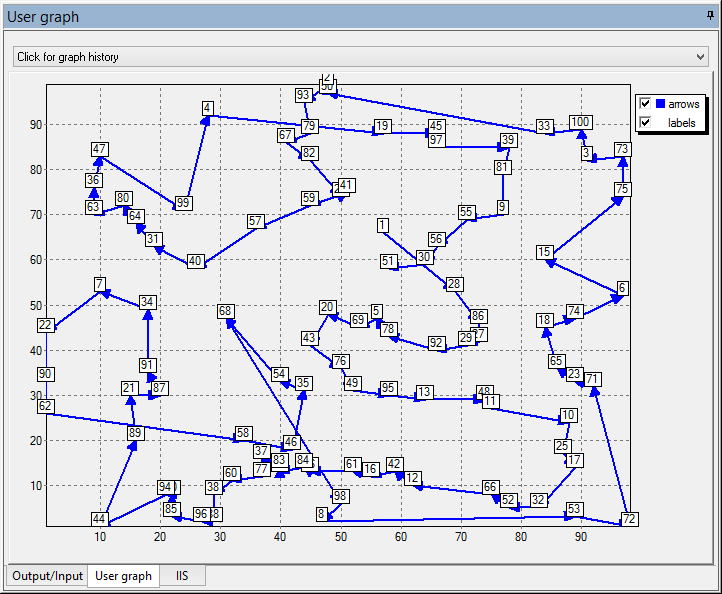
\includegraphics[width=1.0\textwidth]{sa_tsp_100_1.png}
\end{figure}

\end{document}
